% Options for packages loaded elsewhere
\PassOptionsToPackage{unicode}{hyperref}
\PassOptionsToPackage{hyphens}{url}
%
\documentclass[
  12pt,
]{article}
\title{Exploring the Determinants of Biogas Generation Potential in
California}
\usepackage{etoolbox}
\makeatletter
\providecommand{\subtitle}[1]{% add subtitle to \maketitle
  \apptocmd{\@title}{\par {\large #1 \par}}{}{}
}
\makeatother
\subtitle{Web address for GitHub repository}
\author{Jibikeoluwa Faborode, Yinan Ding, Abhay Rao}
\date{}

\usepackage{amsmath,amssymb}
\usepackage{lmodern}
\usepackage{iftex}
\ifPDFTeX
  \usepackage[T1]{fontenc}
  \usepackage[utf8]{inputenc}
  \usepackage{textcomp} % provide euro and other symbols
\else % if luatex or xetex
  \usepackage{unicode-math}
  \defaultfontfeatures{Scale=MatchLowercase}
  \defaultfontfeatures[\rmfamily]{Ligatures=TeX,Scale=1}
  \setmainfont[]{Times New Roman}
\fi
% Use upquote if available, for straight quotes in verbatim environments
\IfFileExists{upquote.sty}{\usepackage{upquote}}{}
\IfFileExists{microtype.sty}{% use microtype if available
  \usepackage[]{microtype}
  \UseMicrotypeSet[protrusion]{basicmath} % disable protrusion for tt fonts
}{}
\makeatletter
\@ifundefined{KOMAClassName}{% if non-KOMA class
  \IfFileExists{parskip.sty}{%
    \usepackage{parskip}
  }{% else
    \setlength{\parindent}{0pt}
    \setlength{\parskip}{6pt plus 2pt minus 1pt}}
}{% if KOMA class
  \KOMAoptions{parskip=half}}
\makeatother
\usepackage{xcolor}
\IfFileExists{xurl.sty}{\usepackage{xurl}}{} % add URL line breaks if available
\IfFileExists{bookmark.sty}{\usepackage{bookmark}}{\usepackage{hyperref}}
\hypersetup{
  pdftitle={Exploring the Determinants of Biogas Generation Potential in California},
  pdfauthor={Jibikeoluwa Faborode, Yinan Ding, Abhay Rao},
  hidelinks,
  pdfcreator={LaTeX via pandoc}}
\urlstyle{same} % disable monospaced font for URLs
\usepackage[margin=2.54cm]{geometry}
\usepackage{graphicx}
\makeatletter
\def\maxwidth{\ifdim\Gin@nat@width>\linewidth\linewidth\else\Gin@nat@width\fi}
\def\maxheight{\ifdim\Gin@nat@height>\textheight\textheight\else\Gin@nat@height\fi}
\makeatother
% Scale images if necessary, so that they will not overflow the page
% margins by default, and it is still possible to overwrite the defaults
% using explicit options in \includegraphics[width, height, ...]{}
\setkeys{Gin}{width=\maxwidth,height=\maxheight,keepaspectratio}
% Set default figure placement to htbp
\makeatletter
\def\fps@figure{htbp}
\makeatother
\setlength{\emergencystretch}{3em} % prevent overfull lines
\providecommand{\tightlist}{%
  \setlength{\itemsep}{0pt}\setlength{\parskip}{0pt}}
\setcounter{secnumdepth}{5}
\ifLuaTeX
  \usepackage{selnolig}  % disable illegal ligatures
\fi

\begin{document}
\maketitle

\newpage
\tableofcontents 
\newpage
\listoftables 
\newpage
\listoffigures 
\newpage

\hypertarget{rationale-and-research-questions}{%
\section{Rationale and Research
Questions}\label{rationale-and-research-questions}}

Methane's global warming potential is estimated to be over 25 times as
potent as that of Carbon Dioxide. The
\href{https://unece.org/challenge\#:~:text=Methane\%20is\%20a\%20powerful\%20greenhouses,grows\%20to\%2084\%2D86\%20times.}{UNECE}
estimates that over a 20 year period, this ratio increases to 84-86
times. Methane is generated from various sources, including (but not
limited to) wastewater treatment, animal manure, landfills, industrial
organic waste.

The NREL estimates that California has the highest biogas generation
potential in the US. According to the
\href{chrome-extension://efaidnbmnnnibpcajpcglclefindmkaj/viewer.html?pdfurl=https\%3A\%2F\%2Famericanbiogascouncil.org\%2Fwp-content\%2Fuploads\%2F2019\%2F05\%2FABCBiogasStateProfile_CA.pdf\&clen=226298\&chunk=true}{American
Biogas Council}, California can power nearly 200,000 homes if this
biogas is utilized appropriately.

We therefore set to find out more about biogas generation potential in
California:

\emph{Firstly, was biogas generation potential correlated with densely
populated areas?} That is, could biogas be channeled to nearby use cases
frequently?

\emph{Secondly, are there additional factors to consider?}

\newpage

\hypertarget{dataset-information}{%
\section{Dataset Information}\label{dataset-information}}

We drew upon two datasets:

\begin{enumerate}
\def\labelenumi{\arabic{enumi}.}
\item
  The National Renewable Energy Laboratory's dataset on methane
  generation potential in the United States of America. This considered
  all US States' CH4 generation potential in metric tons across the
  following sources: landfills, industrial organic waste, animal manure,
  and wastewater, aggregated into Total CH4 potential. This data is
  sourced from 2009-2012.
\item
  The CDC and ATSDR's social vulnerability index, from which we obtained
  county-wide population data, and details on impoverished populations.
  This data is sourced from 2017-2018.
\end{enumerate}

\newpage

\hypertarget{exploratory-analysis}{%
\section{Exploratory Analysis}\label{exploratory-analysis}}

We wrangled and joined both datasets to have a unified, county-wise
dataframe that included data on methane generation potential, population
and poverty. We started our analysis with a visual assessment of spatial
data, to determine if any trends immediately emerged.

Visually, the most populated area of California, given by the county
shaded yellow, Los Angeles, has the highest CH4 generation potential.
The density of impoverished population appears to be similarly
distributed.

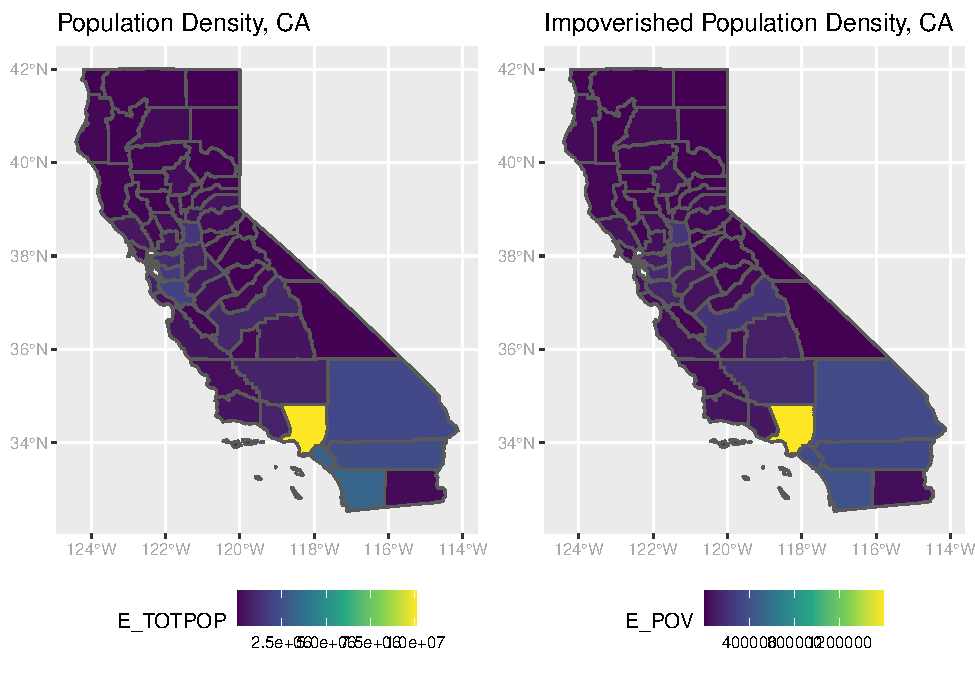
\includegraphics{FDR_ProjectReport_files/figure-latex/unnamed-chunk-2-1.pdf}

Total CH4 generation potential is greatest at the most densely populated
areas. This trend appears to continue with wastewater derived methane.

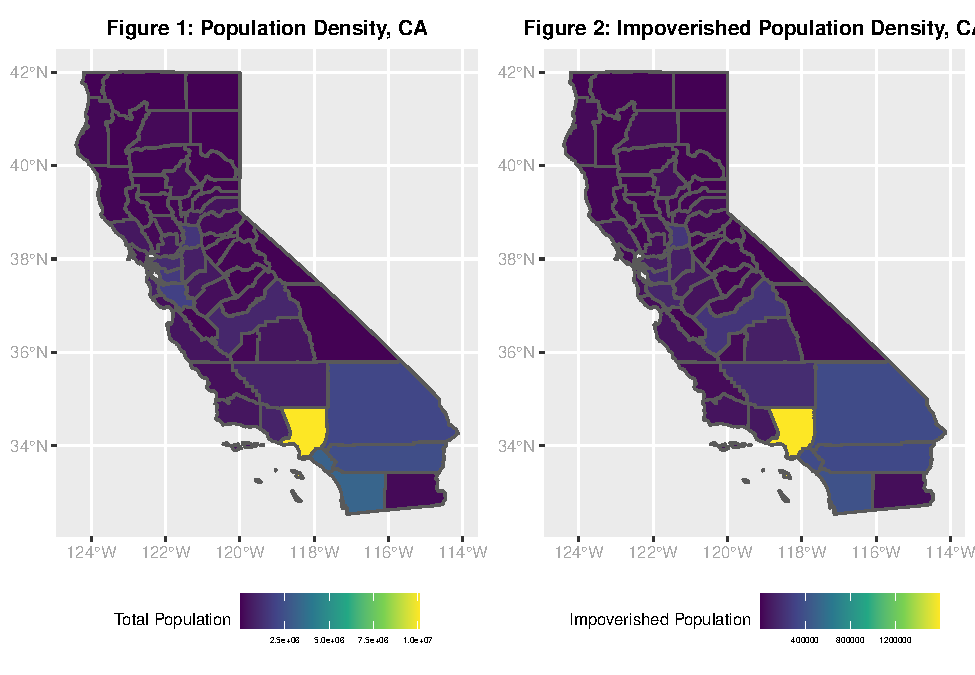
\includegraphics{FDR_ProjectReport_files/figure-latex/unnamed-chunk-3-1.pdf}

Industrial Organic waste, like wastewater, is highly correlated with
population.With landfill-based methane, some counties in central CA,
which do not appear to have a high population, have comparatively high
methane generation potential. There may be some non-population related
factors in play.
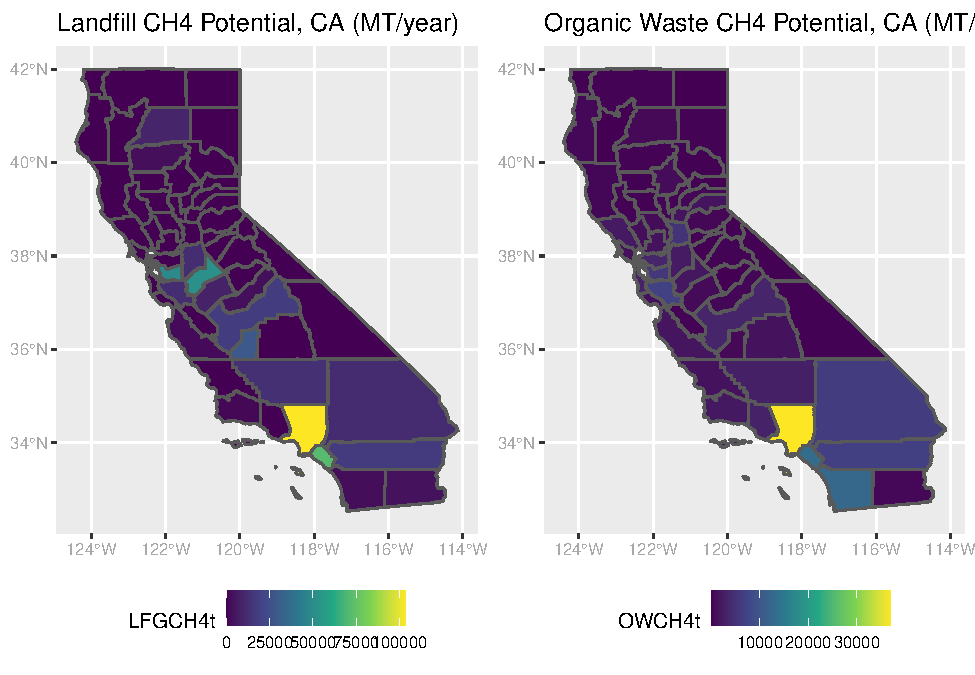
\includegraphics{FDR_ProjectReport_files/figure-latex/unnamed-chunk-4-1.pdf}

The trend with animal-manure derived CH4 however substantially differs
from the previous cases. Population does not appear to be a decisive
factor.

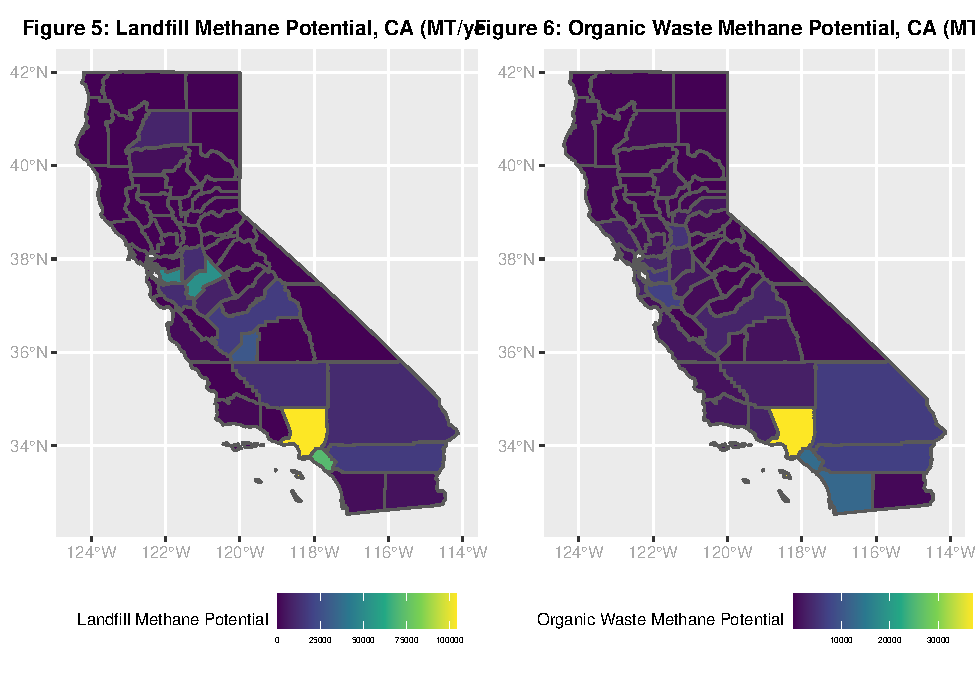
\includegraphics{FDR_ProjectReport_files/figure-latex/unnamed-chunk-5-1.pdf}

\newpage

\hypertarget{analysis}{%
\section{Analysis}\label{analysis}}

\hypertarget{question-1-insert-specific-question-here-and-add-additional-subsections-for-additional-questions-below-if-needed}{%
\subsection{Question 1: \textless insert specific question here and add
additional subsections for additional questions below, if
needed\textgreater{}}\label{question-1-insert-specific-question-here-and-add-additional-subsections-for-additional-questions-below-if-needed}}

\hypertarget{question-2-is-there-a-relationship-between-methane-generation-potential-and-impoverished-populations}{%
\subsection{Question 2: Is there a relationship between methane
generation potential and impoverished
populations?}\label{question-2-is-there-a-relationship-between-methane-generation-potential-and-impoverished-populations}}

\begin{verbatim}
## `geom_smooth()` using formula 'y ~ x'
\end{verbatim}

\begin{verbatim}
## Warning: Removed 1 rows containing non-finite values (stat_smooth).
\end{verbatim}

\begin{verbatim}
## Warning: Removed 1 rows containing missing values (geom_point).
\end{verbatim}

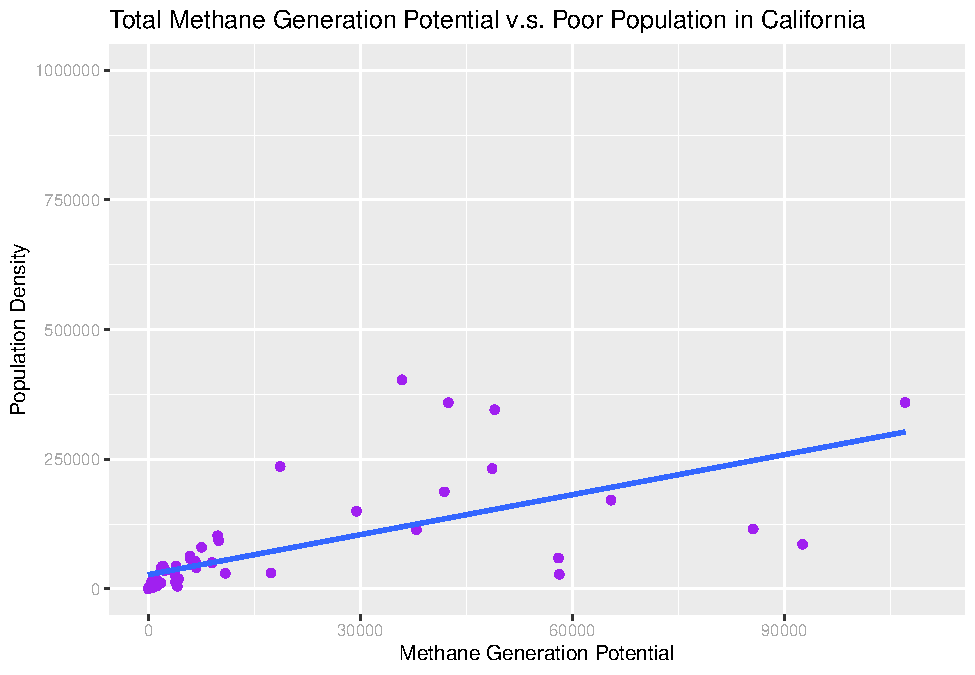
\includegraphics{FDR_ProjectReport_files/figure-latex/unnamed-chunk-7-1.pdf}

\begin{verbatim}
## `geom_smooth()` using formula 'y ~ x'
\end{verbatim}

\begin{verbatim}
## Warning: Removed 1 rows containing non-finite values (stat_smooth).

## Warning: Removed 1 rows containing missing values (geom_point).
\end{verbatim}

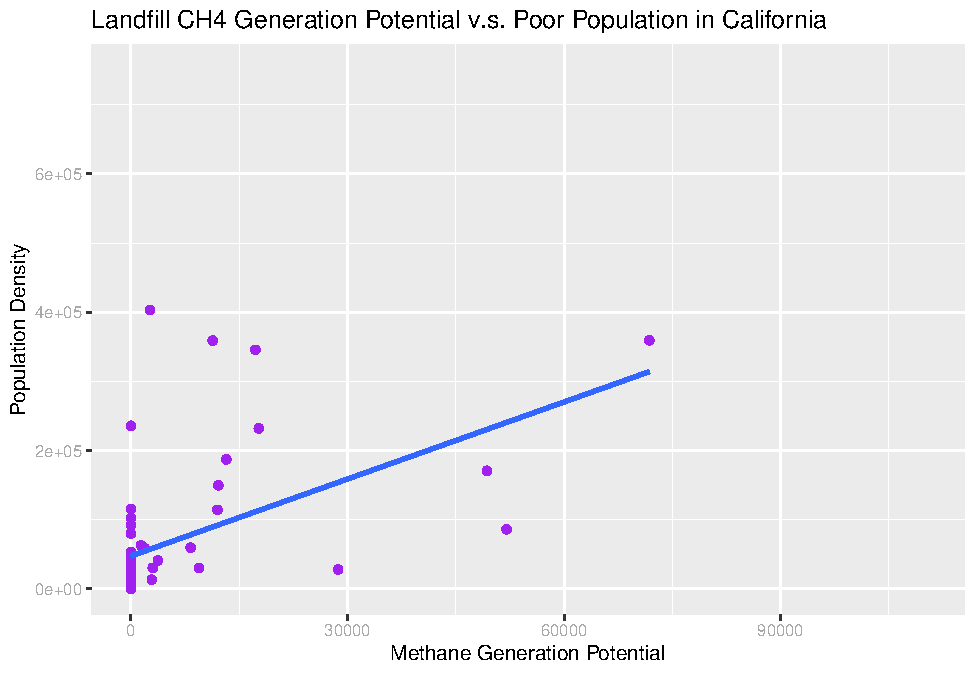
\includegraphics{FDR_ProjectReport_files/figure-latex/unnamed-chunk-7-2.pdf}

\begin{verbatim}
## `geom_smooth()` using formula 'y ~ x'
\end{verbatim}

\begin{verbatim}
## Warning: Removed 1 rows containing non-finite values (stat_smooth).

## Warning: Removed 1 rows containing missing values (geom_point).
\end{verbatim}

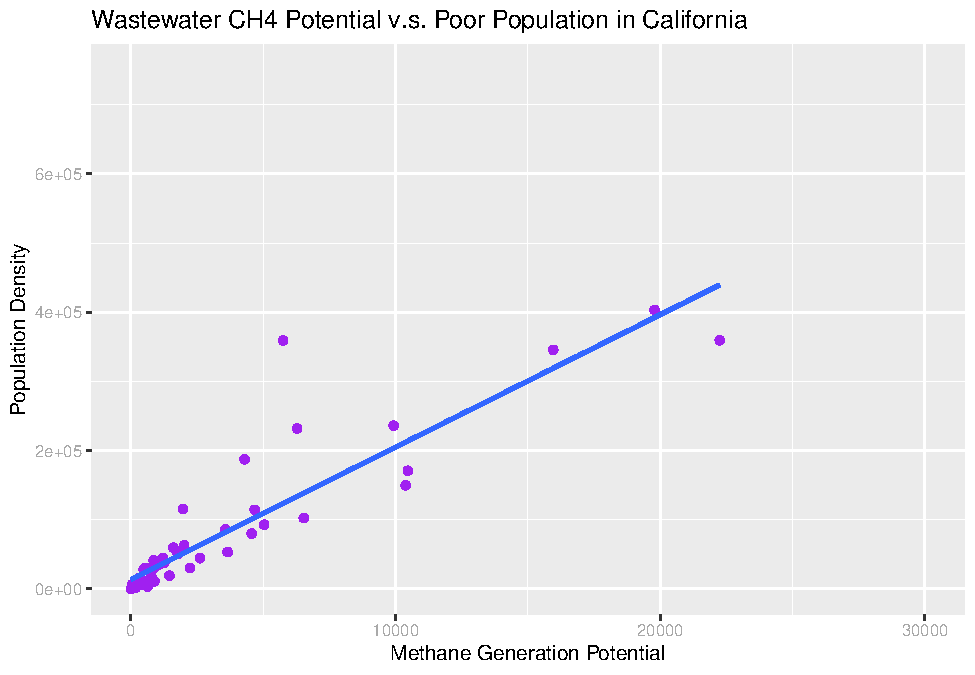
\includegraphics{FDR_ProjectReport_files/figure-latex/unnamed-chunk-7-3.pdf}

\begin{verbatim}
## `geom_smooth()` using formula 'y ~ x'
\end{verbatim}

\begin{verbatim}
## Warning: Removed 1 rows containing non-finite values (stat_smooth).

## Warning: Removed 1 rows containing missing values (geom_point).
\end{verbatim}

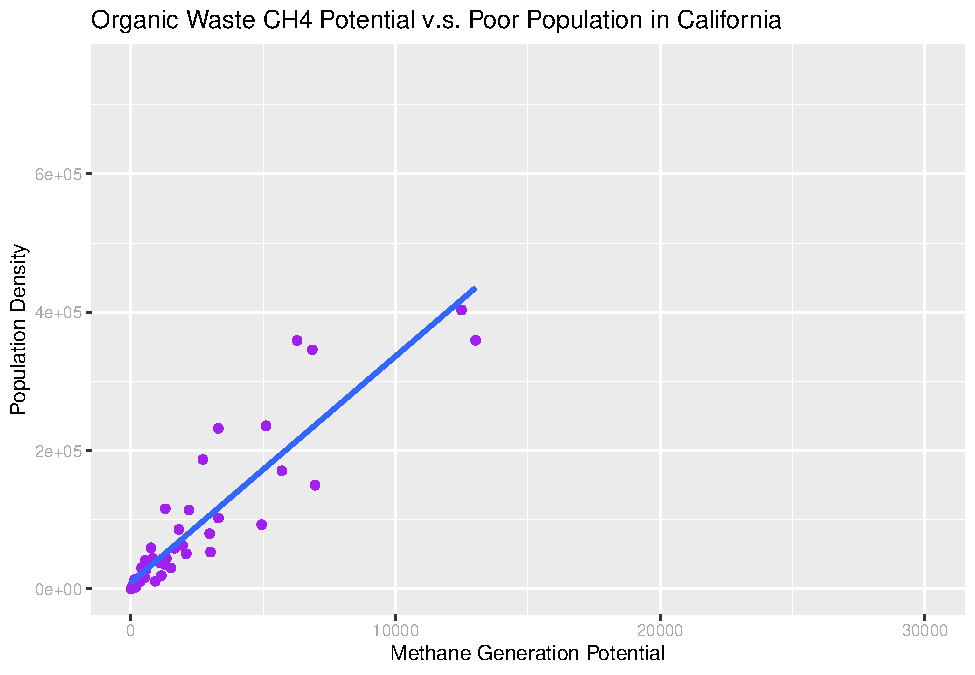
\includegraphics{FDR_ProjectReport_files/figure-latex/unnamed-chunk-7-4.pdf}

\begin{verbatim}
## `geom_smooth()` using formula 'y ~ x'
\end{verbatim}

\begin{verbatim}
## Warning: Removed 2 rows containing non-finite values (stat_smooth).
\end{verbatim}

\begin{verbatim}
## Warning: Removed 2 rows containing missing values (geom_point).
\end{verbatim}

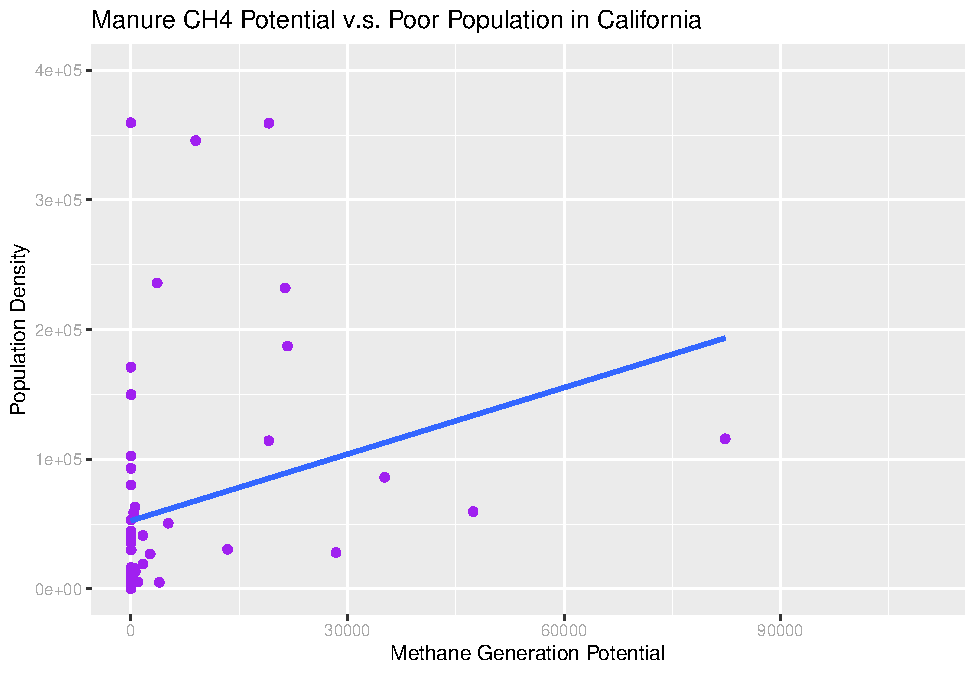
\includegraphics{FDR_ProjectReport_files/figure-latex/unnamed-chunk-7-5.pdf}

\newpage

\hypertarget{summary-and-conclusions}{%
\section{Summary and Conclusions}\label{summary-and-conclusions}}

\newpage

\hypertarget{references}{%
\section{References}\label{references}}

\textless add references here if relevant, otherwise delete this
section\textgreater{}

\end{document}
